  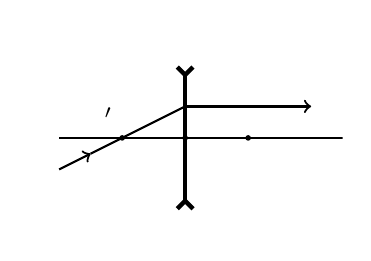
\begin{tikzpicture}[scale=0.4]
    \clip (-5,-3) rectangle (5,3.5) ; %Les dimensions de l'image
    %\draw [help lines] (-4,-3) grid [step=0.5] (8,2.5) ; %% Le quadrillage
    \draw [->,thick] (-4,0) -- (8,0) ; %% L'axe optique
    \draw [ultra thick] (0,-2) -- (0,2)  ; %% Le corps du système 
    
    \draw [ultra thick] (-0.25,-2.25) -- (0,-2) -- (0.25,-2.25)
                         (-0.25,2.25) -- (0,2) -- (0.25,2.25) ;                    %La lentille divergente

    \filldraw [black] (0,0) circle (2pt) node [above right] {$\ptO$} ;  %Le centre optique
    \filldraw [black] (2.0,0) circle (2pt) node [above right] {$\ptF$}; %Le foyer objet
    \filldraw [black] (-2.0,0) circle (2pt) node [above left] {$\ptF'$} ; %Le foyer image
    
    \draw [->,thick] (-4,-1) -- (-3,-0.5) ; 
     \draw [-,thick] (-3,-0.5) -- (0,1) ;  %Le rayon incident
    \draw [->,thick] (0,1) -- (4,1) ; %Le rayon émergent
      
  \end{tikzpicture}